\begin{quote}
``Praxis, a noble activity, is always one of use, as distinct from
poesis which designates fabrication. Only the former, which plays and
acts, but does not produce, is noble.'' {[}1{]} (p. 101)
\end{quote}
\begin{figure}
\centering
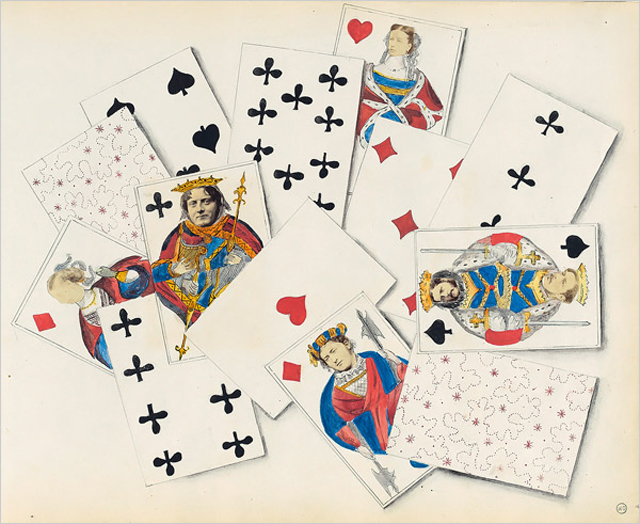
\includegraphics[width=.8\textwidth]{../pictures/collage.jpg}
\caption*{19th century collage cards, care of
  \href{http://www.nickhaus.com/2010/02/afternoon-remembered-complete-with.html}{Nick
    Haus}}
\end{figure}


There is a tension between ``making stuff'' (\emph{poesis}) and ``using
stuff'' (\emph{praxis}). Peer \emph{production}, as the name indicates,
is about ``making stuff.'' And making stuff can be fun. But we should
also ask ourselves, how much new stuff do we really need? There's not a
hard and fast answer to that. We should also consider how much
``learning'' is really ``remix'' -- that is, re-use and recycling of
other people's ideas and techniques. Understanding and negotiating the
tension between reuse and creativity is the key to \emph{the art of
remix} or ``paragogical praxis''!

\subsubsection{Reference}

\begin{enumerate}
\item
  Baudrillard, J. (1975). \emph{The mirror of production}. Telos Press
\end{enumerate}
